\section{Messungen mit Audio Precision (System Two Cascade)}
\subsection{Messung des Quantisierungsrauschens}
\subsubsection{Aufgabenstellung}
Messung des Quantisierungsrauschens (SNR) am Mischpult D/A Umsetzer (Line Ausgang des Lawo $mc^266$) mit $14-20$Bit Auflösung, Schrittweite 1 Bit. Vergleichen Sie mit den erwarteten Werten. Was kann aus den Messergebnissen gefolgert werden?

\subsubsection{Messaufbau}

\subsubsection{Formeln}

\subsubsection{Berechnungsbeispiele}

\subsubsection{Diagramme}

\subsubsection{Diskussion}


\subsection{Messung mit Jitter}
\subsubsection{Aufgabenstellung}
\begin{enumerate}
\item Messung der FFT-Spektren verjitterter Signale. Untersuchung für verschiedene Jitterfrequenzen und verschiedene Signalfrequenzen.
\item Vergrößerung der Jitteramplitude, bis die Übertragung zusammenbricht.
\item Aufzeichnung der THD+N - Kennlinie bei Vergrößerung der Jitteramplitude bei den Jitterfrequenzen $500$Hz, $5$kHz und $10$kHz. 
\end{enumerate}

\subsubsection{Messaufbau}

\subsubsection{Formeln}

\subsubsection{Berechnungsbeispiele}

\subsubsection{Diagramme}

\begin{figure}[h!]
\centering
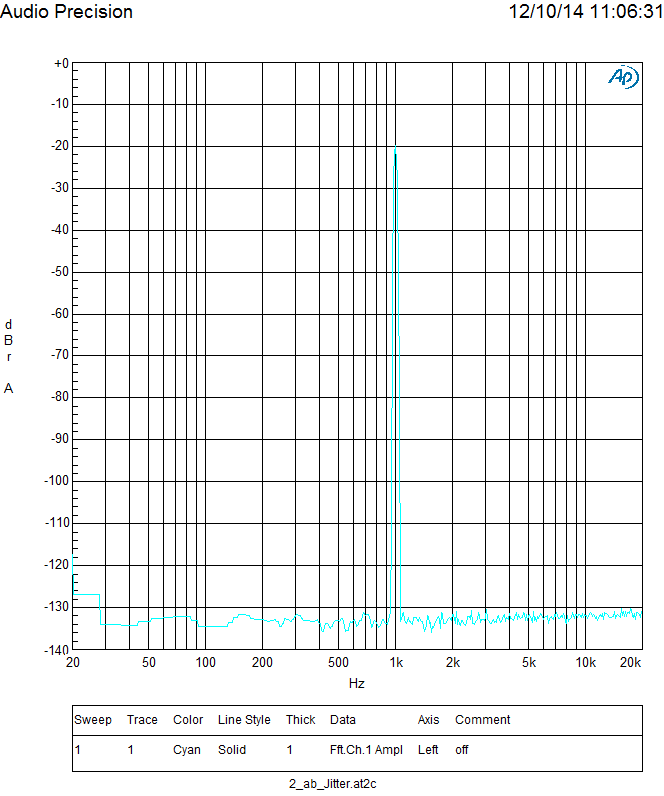
\includegraphics[width=\columnwidth]{figures/Aufg2/off_1khz.PNG} 
\caption{Test}
\end{figure}


\begin{figure}[h!]
\centering
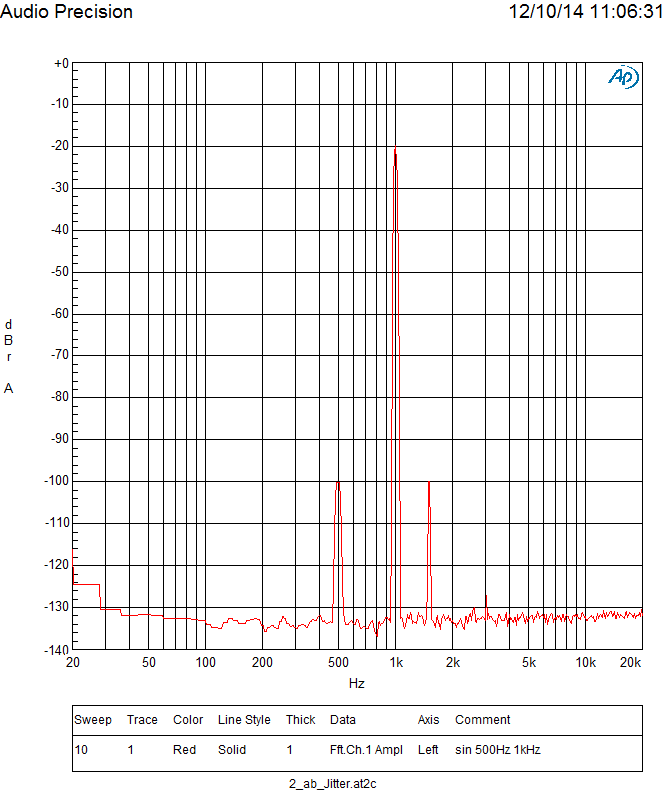
\includegraphics[width=\columnwidth]{figures/Aufg2/10.PNG} 
\caption{Test}
\end{figure}

\begin{figure}[h!]
\centering
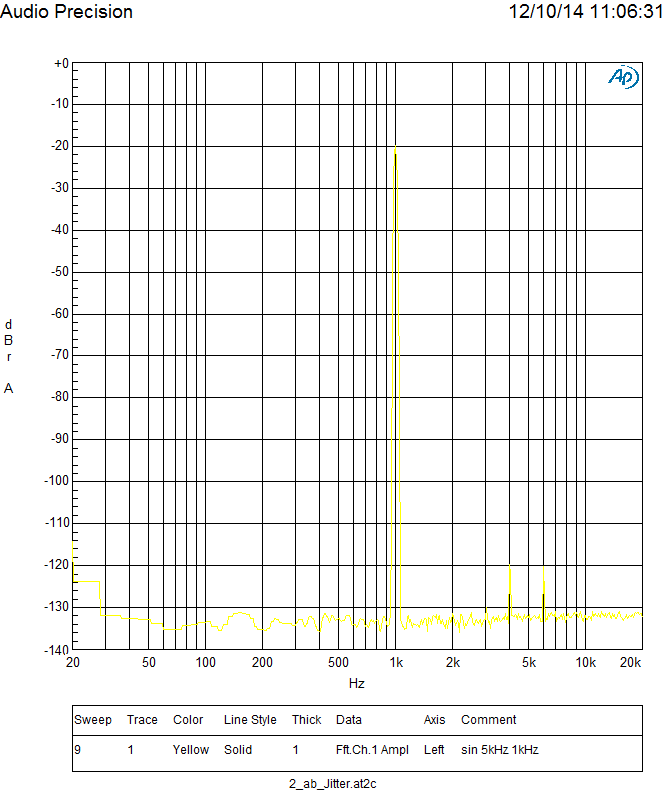
\includegraphics[width=\columnwidth]{figures/Aufg2/9.PNG} 
\caption{Test}
\end{figure}

\begin{figure}[h!]
\centering
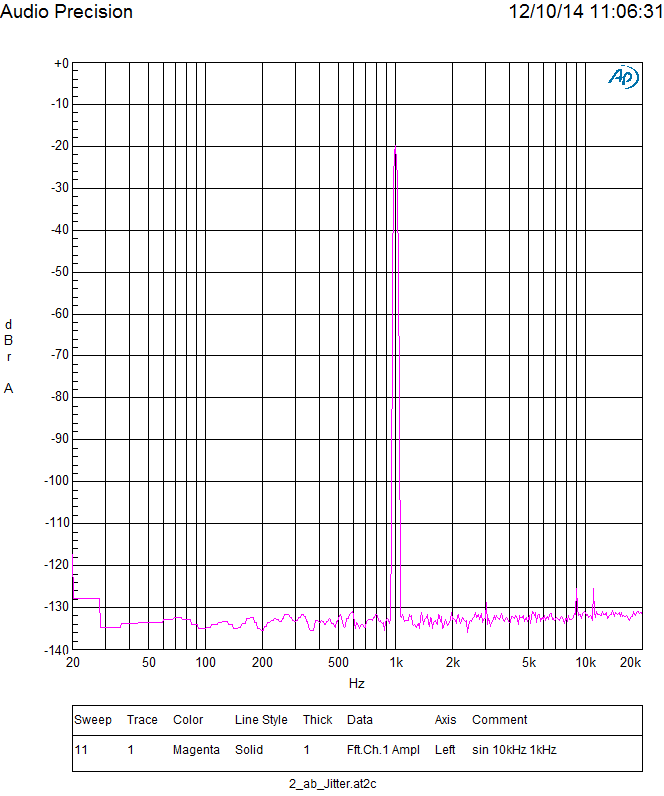
\includegraphics[width=\columnwidth]{figures/Aufg2/11.PNG} 
\caption{Test}
\end{figure}


\begin{figure}[h!]
\centering
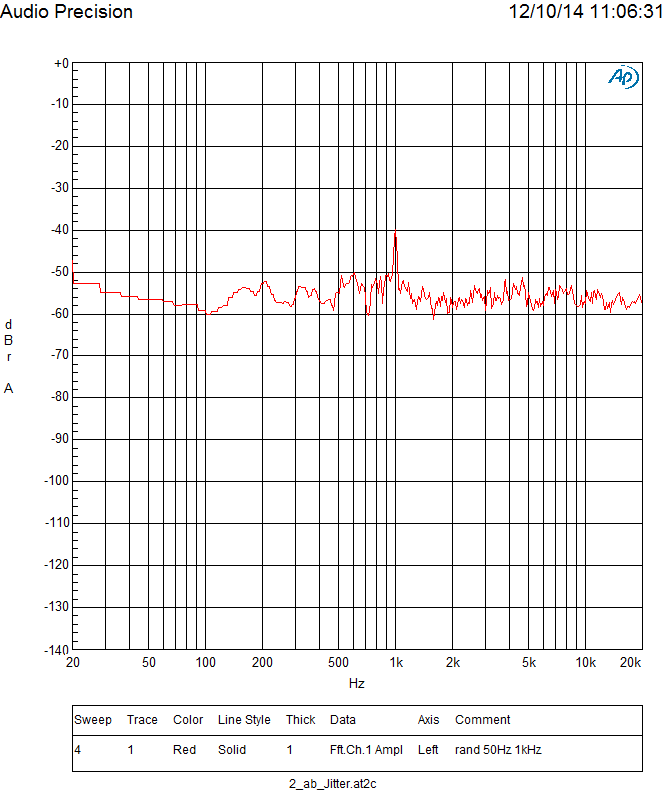
\includegraphics[width=\columnwidth]{figures/Aufg2/4.PNG} 
\caption{Test}
\end{figure}
\clearpage

\subsubsection{Diskussion}

\subsection{Klirrfaktor}
\subsubsection{Aufgabenstellung}
\begin{enumerate}
\item Messen einer THD+N-Kennlinie über den Dynamikbereich mit und ohne Dither
\item Messen einer THD+N-Kennlinie über der Frequenz mit und ohne Dither
\end{enumerate}

\subsubsection{Messaufbau}

\subsubsection{Formeln}

\subsubsection{Berechnungsbeispiele}

\subsubsection{Diagramme}
\begin{figure}[h!]
\centering
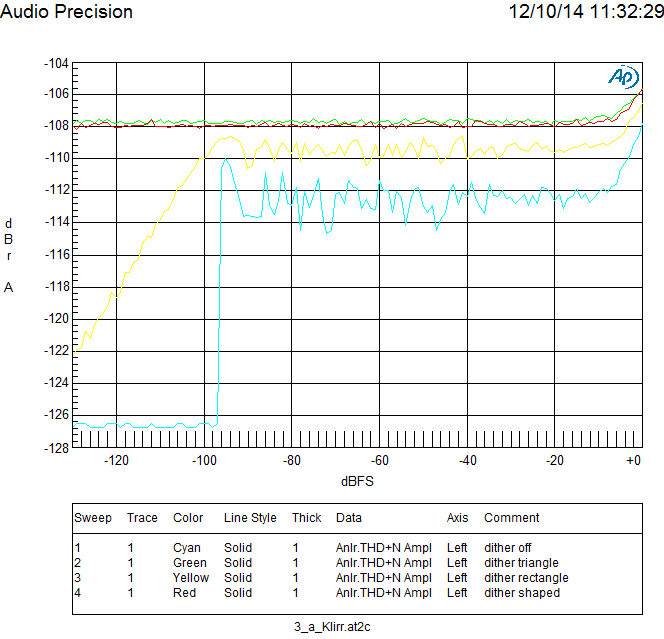
\includegraphics[width=\columnwidth]{figures/Aufg2/3a5.PNG} 
\caption{Test}
\end{figure}

\begin{figure}[h!]
\centering
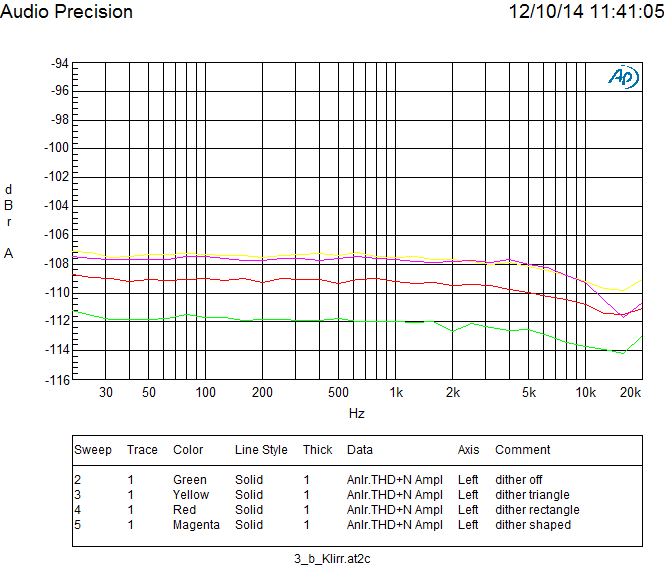
\includegraphics[width=\columnwidth]{figures/Aufg2/3b1.PNG} 
\caption{Test}
\end{figure}
\clearpage
\subsubsection{Diskussion}


\subsection{Geräteliste}


